% Created by tikzDevice version 0.12.6 on 2025-04-07 03:17:30
% !TEX encoding = UTF-8 Unicode
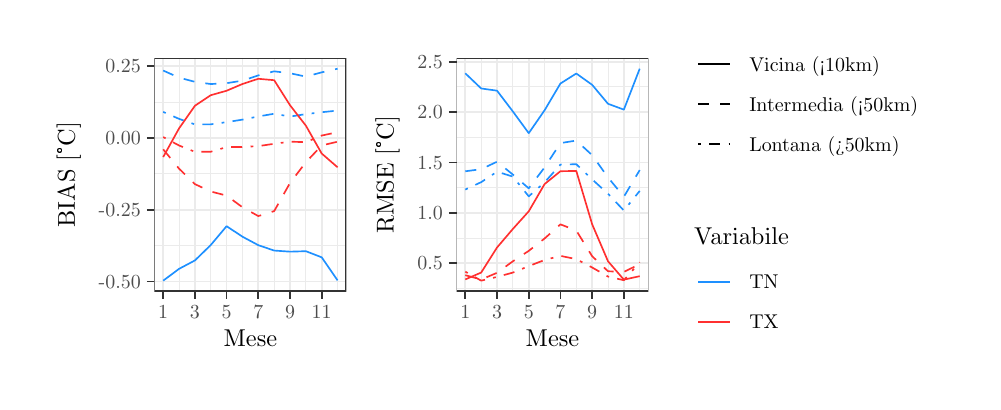
\begin{tikzpicture}[x=1pt,y=1pt]
\definecolor{fillColor}{RGB}{255,255,255}
\path[use as bounding box,fill=fillColor] (0,0) rectangle (341.43,128.04);
\begin{scope}
\path[clip] (  0.00,  0.00) rectangle (341.43,128.04);
\definecolor{drawColor}{RGB}{255,255,255}

\path[draw=drawColor,line width= 0.6pt,line join=round,line cap=round,fill=fillColor] (  0.00,  0.00) rectangle (341.43,128.04);
\end{scope}
\begin{scope}
\path[clip] (  5.50,  5.50) rectangle (120.63,122.54);
\definecolor{drawColor}{RGB}{255,255,255}
\definecolor{fillColor}{RGB}{255,255,255}

\path[draw=drawColor,line width= 0.6pt,line join=round,line cap=round,fill=fillColor] (  5.50,  5.50) rectangle (120.63,122.54);
\end{scope}
\begin{scope}
\path[clip] (120.63,  5.50) rectangle (335.93,122.54);
\definecolor{drawColor}{RGB}{255,255,255}
\definecolor{fillColor}{RGB}{255,255,255}

\path[draw=drawColor,line width= 0.6pt,line join=round,line cap=round,fill=fillColor] (120.63,  5.50) rectangle (335.93,122.54);
\end{scope}
\begin{scope}
\path[clip] ( 45.82, 32.79) rectangle (115.13,117.04);
\definecolor{fillColor}{RGB}{255,255,255}

\path[fill=fillColor] ( 45.82, 32.79) rectangle (115.13,117.04);
\definecolor{drawColor}{gray}{0.92}

\path[draw=drawColor,line width= 0.3pt,line join=round] ( 45.82, 49.27) --
	(115.13, 49.27);

\path[draw=drawColor,line width= 0.3pt,line join=round] ( 45.82, 75.22) --
	(115.13, 75.22);

\path[draw=drawColor,line width= 0.3pt,line join=round] ( 45.82,101.17) --
	(115.13,101.17);

\path[draw=drawColor,line width= 0.3pt,line join=round] ( 54.70, 32.79) --
	( 54.70,117.04);

\path[draw=drawColor,line width= 0.3pt,line join=round] ( 66.15, 32.79) --
	( 66.15,117.04);

\path[draw=drawColor,line width= 0.3pt,line join=round] ( 77.61, 32.79) --
	( 77.61,117.04);

\path[draw=drawColor,line width= 0.3pt,line join=round] ( 89.07, 32.79) --
	( 89.07,117.04);

\path[draw=drawColor,line width= 0.3pt,line join=round] (100.53, 32.79) --
	(100.53,117.04);

\path[draw=drawColor,line width= 0.3pt,line join=round] (111.98, 32.79) --
	(111.98,117.04);

\path[draw=drawColor,line width= 0.6pt,line join=round] ( 45.82, 36.30) --
	(115.13, 36.30);

\path[draw=drawColor,line width= 0.6pt,line join=round] ( 45.82, 62.25) --
	(115.13, 62.25);

\path[draw=drawColor,line width= 0.6pt,line join=round] ( 45.82, 88.20) --
	(115.13, 88.20);

\path[draw=drawColor,line width= 0.6pt,line join=round] ( 45.82,114.15) --
	(115.13,114.15);

\path[draw=drawColor,line width= 0.6pt,line join=round] ( 48.97, 32.79) --
	( 48.97,117.04);

\path[draw=drawColor,line width= 0.6pt,line join=round] ( 60.43, 32.79) --
	( 60.43,117.04);

\path[draw=drawColor,line width= 0.6pt,line join=round] ( 71.88, 32.79) --
	( 71.88,117.04);

\path[draw=drawColor,line width= 0.6pt,line join=round] ( 83.34, 32.79) --
	( 83.34,117.04);

\path[draw=drawColor,line width= 0.6pt,line join=round] ( 94.80, 32.79) --
	( 94.80,117.04);

\path[draw=drawColor,line width= 0.6pt,line join=round] (106.25, 32.79) --
	(106.25,117.04);
\definecolor{drawColor}{RGB}{30,144,255}

\path[draw=drawColor,line width= 0.6pt,line join=round] ( 48.97, 36.62) --
	( 54.70, 40.89) --
	( 60.43, 43.93) --
	( 66.15, 49.49) --
	( 71.88, 56.31) --
	( 77.61, 52.51) --
	( 83.34, 49.45) --
	( 89.07, 47.50) --
	( 94.80, 47.10) --
	(100.53, 47.27) --
	(106.25, 45.05) --
	(111.98, 36.73);

\path[draw=drawColor,line width= 0.6pt,dash pattern=on 4pt off 4pt ,line join=round] ( 48.97,112.54) --
	( 54.70,109.99) --
	( 60.43,108.47) --
	( 66.15,107.67) --
	( 71.88,107.98) --
	( 77.61,108.90) --
	( 83.34,110.80) --
	( 89.07,112.26) --
	( 94.80,111.58) --
	(100.53,110.35) --
	(106.25,111.90) --
	(111.98,113.21);

\path[draw=drawColor,line width= 0.6pt,dash pattern=on 1pt off 3pt on 4pt off 3pt ,line join=round] ( 48.97, 97.60) --
	( 54.70, 95.09) --
	( 60.43, 93.09) --
	( 66.15, 93.11) --
	( 71.88, 93.90) --
	( 77.61, 94.81) --
	( 83.34, 95.96) --
	( 89.07, 96.94) --
	( 94.80, 95.92) --
	(100.53, 96.80) --
	(106.25, 97.49) --
	(111.98, 98.08);
\definecolor{drawColor}{RGB}{255,48,48}

\path[draw=drawColor,line width= 0.6pt,line join=round] ( 48.97, 81.30) --
	( 54.70, 91.64) --
	( 60.43, 99.81) --
	( 66.15,103.63) --
	( 71.88,105.25) --
	( 77.61,107.69) --
	( 83.34,109.57) --
	( 89.07,109.06) --
	( 94.80,100.01) --
	(100.53, 92.63) --
	(106.25, 82.56) --
	(111.98, 77.59);

\path[draw=drawColor,line width= 0.6pt,dash pattern=on 4pt off 4pt ,line join=round] ( 48.97, 84.08) --
	( 54.70, 77.09) --
	( 60.43, 71.51) --
	( 66.15, 68.84) --
	( 71.88, 67.36) --
	( 77.61, 63.14) --
	( 83.34, 59.96) --
	( 89.07, 61.75) --
	( 94.80, 71.93) --
	(100.53, 79.42) --
	(106.25, 85.48) --
	(111.98, 86.84);

\path[draw=drawColor,line width= 0.6pt,dash pattern=on 1pt off 3pt on 4pt off 3pt ,line join=round] ( 48.97, 88.51) --
	( 54.70, 85.47) --
	( 60.43, 83.18) --
	( 66.15, 83.21) --
	( 71.88, 84.88) --
	( 77.61, 84.95) --
	( 83.34, 85.24) --
	( 89.07, 86.08) --
	( 94.80, 86.85) --
	(100.53, 86.66) --
	(106.25, 89.06) --
	(111.98, 90.27);
\definecolor{drawColor}{gray}{0.20}

\path[draw=drawColor,line width= 0.6pt,line join=round,line cap=round] ( 45.82, 32.79) rectangle (115.13,117.04);
\end{scope}
\begin{scope}
\path[clip] (  0.00,  0.00) rectangle (341.43,128.04);
\definecolor{drawColor}{gray}{0.30}

\node[text=drawColor,anchor=base east,inner sep=0pt, outer sep=0pt, scale=  0.72] at ( 40.87, 33.84) {-0.50};

\node[text=drawColor,anchor=base east,inner sep=0pt, outer sep=0pt, scale=  0.72] at ( 40.87, 59.79) {-0.25};

\node[text=drawColor,anchor=base east,inner sep=0pt, outer sep=0pt, scale=  0.72] at ( 40.87, 85.74) {0.00};

\node[text=drawColor,anchor=base east,inner sep=0pt, outer sep=0pt, scale=  0.72] at ( 40.87,111.68) {0.25};
\end{scope}
\begin{scope}
\path[clip] (  0.00,  0.00) rectangle (341.43,128.04);
\definecolor{drawColor}{gray}{0.20}

\path[draw=drawColor,line width= 0.6pt,line join=round] ( 43.07, 36.30) --
	( 45.82, 36.30);

\path[draw=drawColor,line width= 0.6pt,line join=round] ( 43.07, 62.25) --
	( 45.82, 62.25);

\path[draw=drawColor,line width= 0.6pt,line join=round] ( 43.07, 88.20) --
	( 45.82, 88.20);

\path[draw=drawColor,line width= 0.6pt,line join=round] ( 43.07,114.15) --
	( 45.82,114.15);
\end{scope}
\begin{scope}
\path[clip] (  0.00,  0.00) rectangle (341.43,128.04);
\definecolor{drawColor}{gray}{0.20}

\path[draw=drawColor,line width= 0.6pt,line join=round] ( 48.97, 30.04) --
	( 48.97, 32.79);

\path[draw=drawColor,line width= 0.6pt,line join=round] ( 60.43, 30.04) --
	( 60.43, 32.79);

\path[draw=drawColor,line width= 0.6pt,line join=round] ( 71.88, 30.04) --
	( 71.88, 32.79);

\path[draw=drawColor,line width= 0.6pt,line join=round] ( 83.34, 30.04) --
	( 83.34, 32.79);

\path[draw=drawColor,line width= 0.6pt,line join=round] ( 94.80, 30.04) --
	( 94.80, 32.79);

\path[draw=drawColor,line width= 0.6pt,line join=round] (106.25, 30.04) --
	(106.25, 32.79);
\end{scope}
\begin{scope}
\path[clip] (  0.00,  0.00) rectangle (341.43,128.04);
\definecolor{drawColor}{gray}{0.30}

\node[text=drawColor,anchor=base,inner sep=0pt, outer sep=0pt, scale=  0.72] at ( 48.97, 22.91) {1};

\node[text=drawColor,anchor=base,inner sep=0pt, outer sep=0pt, scale=  0.72] at ( 60.43, 22.91) {3};

\node[text=drawColor,anchor=base,inner sep=0pt, outer sep=0pt, scale=  0.72] at ( 71.88, 22.91) {5};

\node[text=drawColor,anchor=base,inner sep=0pt, outer sep=0pt, scale=  0.72] at ( 83.34, 22.91) {7};

\node[text=drawColor,anchor=base,inner sep=0pt, outer sep=0pt, scale=  0.72] at ( 94.80, 22.91) {9};

\node[text=drawColor,anchor=base,inner sep=0pt, outer sep=0pt, scale=  0.72] at (106.25, 22.91) {11};
\end{scope}
\begin{scope}
\path[clip] (  0.00,  0.00) rectangle (341.43,128.04);
\definecolor{drawColor}{RGB}{0,0,0}

\node[text=drawColor,anchor=base,inner sep=0pt, outer sep=0pt, scale=  0.88] at ( 80.48, 12.71) {Mese};
\end{scope}
\begin{scope}
\path[clip] (  0.00,  0.00) rectangle (341.43,128.04);
\definecolor{drawColor}{RGB}{0,0,0}

\node[text=drawColor,rotate= 90.00,anchor=base,inner sep=0pt, outer sep=0pt, scale=  0.88] at ( 17.06, 74.91) {BIAS [\textdegree C]};
\end{scope}
\begin{scope}
\path[clip] (154.99, 32.79) rectangle (224.31,117.04);
\definecolor{fillColor}{RGB}{255,255,255}

\path[fill=fillColor] (154.99, 32.79) rectangle (224.31,117.04);
\definecolor{drawColor}{gray}{0.92}

\path[draw=drawColor,line width= 0.3pt,line join=round] (154.99, 33.85) --
	(224.31, 33.85);

\path[draw=drawColor,line width= 0.3pt,line join=round] (154.99, 52.05) --
	(224.31, 52.05);

\path[draw=drawColor,line width= 0.3pt,line join=round] (154.99, 70.25) --
	(224.31, 70.25);

\path[draw=drawColor,line width= 0.3pt,line join=round] (154.99, 88.45) --
	(224.31, 88.45);

\path[draw=drawColor,line width= 0.3pt,line join=round] (154.99,106.64) --
	(224.31,106.64);

\path[draw=drawColor,line width= 0.3pt,line join=round] (163.87, 32.79) --
	(163.87,117.04);

\path[draw=drawColor,line width= 0.3pt,line join=round] (175.33, 32.79) --
	(175.33,117.04);

\path[draw=drawColor,line width= 0.3pt,line join=round] (186.79, 32.79) --
	(186.79,117.04);

\path[draw=drawColor,line width= 0.3pt,line join=round] (198.24, 32.79) --
	(198.24,117.04);

\path[draw=drawColor,line width= 0.3pt,line join=round] (209.70, 32.79) --
	(209.70,117.04);

\path[draw=drawColor,line width= 0.3pt,line join=round] (221.16, 32.79) --
	(221.16,117.04);

\path[draw=drawColor,line width= 0.6pt,line join=round] (154.99, 42.95) --
	(224.31, 42.95);

\path[draw=drawColor,line width= 0.6pt,line join=round] (154.99, 61.15) --
	(224.31, 61.15);

\path[draw=drawColor,line width= 0.6pt,line join=round] (154.99, 79.35) --
	(224.31, 79.35);

\path[draw=drawColor,line width= 0.6pt,line join=round] (154.99, 97.54) --
	(224.31, 97.54);

\path[draw=drawColor,line width= 0.6pt,line join=round] (154.99,115.74) --
	(224.31,115.74);

\path[draw=drawColor,line width= 0.6pt,line join=round] (158.14, 32.79) --
	(158.14,117.04);

\path[draw=drawColor,line width= 0.6pt,line join=round] (169.60, 32.79) --
	(169.60,117.04);

\path[draw=drawColor,line width= 0.6pt,line join=round] (181.06, 32.79) --
	(181.06,117.04);

\path[draw=drawColor,line width= 0.6pt,line join=round] (192.51, 32.79) --
	(192.51,117.04);

\path[draw=drawColor,line width= 0.6pt,line join=round] (203.97, 32.79) --
	(203.97,117.04);

\path[draw=drawColor,line width= 0.6pt,line join=round] (215.43, 32.79) --
	(215.43,117.04);
\definecolor{drawColor}{RGB}{30,144,255}

\path[draw=drawColor,line width= 0.6pt,line join=round] (158.14,111.54) --
	(163.87,106.07) --
	(169.60,105.27) --
	(175.33, 97.75) --
	(181.06, 89.92) --
	(186.79, 98.20) --
	(192.51,107.86) --
	(198.24,111.48) --
	(203.97,107.39) --
	(209.70,100.54) --
	(215.43, 98.42) --
	(221.16,113.21);

\path[draw=drawColor,line width= 0.6pt,dash pattern=on 4pt off 4pt ,line join=round] (158.14, 76.14) --
	(163.87, 76.91) --
	(169.60, 79.60) --
	(175.33, 74.95) --
	(181.06, 69.98) --
	(186.79, 77.56) --
	(192.51, 86.33) --
	(198.24, 87.25) --
	(203.97, 81.97) --
	(209.70, 73.93) --
	(215.43, 66.94) --
	(221.16, 76.58);

\path[draw=drawColor,line width= 0.6pt,dash pattern=on 1pt off 3pt on 4pt off 3pt ,line join=round] (158.14, 69.54) --
	(163.87, 72.22) --
	(169.60, 76.00) --
	(175.33, 74.22) --
	(181.06, 67.09) --
	(186.79, 72.14) --
	(192.51, 78.56) --
	(198.24, 78.70) --
	(203.97, 73.22) --
	(209.70, 68.03) --
	(215.43, 61.97) --
	(221.16, 69.05);
\definecolor{drawColor}{RGB}{255,48,48}

\path[draw=drawColor,line width= 0.6pt,line join=round] (158.14, 37.07) --
	(163.87, 39.55) --
	(169.60, 48.60) --
	(175.33, 55.32) --
	(181.06, 61.67) --
	(186.79, 71.53) --
	(192.51, 76.17) --
	(198.24, 76.27) --
	(203.97, 57.01) --
	(209.70, 43.63) --
	(215.43, 36.99) --
	(221.16, 38.24);

\path[draw=drawColor,line width= 0.6pt,dash pattern=on 4pt off 4pt ,line join=round] (158.14, 38.60) --
	(163.87, 37.03) --
	(169.60, 39.46) --
	(175.33, 43.63) --
	(181.06, 47.39) --
	(186.79, 51.86) --
	(192.51, 56.97) --
	(198.24, 54.74) --
	(203.97, 45.46) --
	(209.70, 40.02) --
	(215.43, 39.77) --
	(221.16, 42.60);

\path[draw=drawColor,line width= 0.6pt,dash pattern=on 1pt off 3pt on 4pt off 3pt ,line join=round] (158.14, 39.87) --
	(163.87, 36.62) --
	(169.60, 37.98) --
	(175.33, 39.54) --
	(181.06, 41.88) --
	(186.79, 44.10) --
	(192.51, 45.58) --
	(198.24, 44.41) --
	(203.97, 41.38) --
	(209.70, 38.10) --
	(215.43, 36.78) --
	(221.16, 43.26);
\definecolor{drawColor}{gray}{0.20}

\path[draw=drawColor,line width= 0.6pt,line join=round,line cap=round] (154.99, 32.79) rectangle (224.31,117.04);
\end{scope}
\begin{scope}
\path[clip] (  0.00,  0.00) rectangle (341.43,128.04);
\definecolor{drawColor}{gray}{0.30}

\node[text=drawColor,anchor=base east,inner sep=0pt, outer sep=0pt, scale=  0.72] at (150.04, 40.49) {0.5};

\node[text=drawColor,anchor=base east,inner sep=0pt, outer sep=0pt, scale=  0.72] at (150.04, 58.68) {1.0};

\node[text=drawColor,anchor=base east,inner sep=0pt, outer sep=0pt, scale=  0.72] at (150.04, 76.88) {1.5};

\node[text=drawColor,anchor=base east,inner sep=0pt, outer sep=0pt, scale=  0.72] at (150.04, 95.08) {2.0};

\node[text=drawColor,anchor=base east,inner sep=0pt, outer sep=0pt, scale=  0.72] at (150.04,113.28) {2.5};
\end{scope}
\begin{scope}
\path[clip] (  0.00,  0.00) rectangle (341.43,128.04);
\definecolor{drawColor}{gray}{0.20}

\path[draw=drawColor,line width= 0.6pt,line join=round] (152.24, 42.95) --
	(154.99, 42.95);

\path[draw=drawColor,line width= 0.6pt,line join=round] (152.24, 61.15) --
	(154.99, 61.15);

\path[draw=drawColor,line width= 0.6pt,line join=round] (152.24, 79.35) --
	(154.99, 79.35);

\path[draw=drawColor,line width= 0.6pt,line join=round] (152.24, 97.54) --
	(154.99, 97.54);

\path[draw=drawColor,line width= 0.6pt,line join=round] (152.24,115.74) --
	(154.99,115.74);
\end{scope}
\begin{scope}
\path[clip] (  0.00,  0.00) rectangle (341.43,128.04);
\definecolor{drawColor}{gray}{0.20}

\path[draw=drawColor,line width= 0.6pt,line join=round] (158.14, 30.04) --
	(158.14, 32.79);

\path[draw=drawColor,line width= 0.6pt,line join=round] (169.60, 30.04) --
	(169.60, 32.79);

\path[draw=drawColor,line width= 0.6pt,line join=round] (181.06, 30.04) --
	(181.06, 32.79);

\path[draw=drawColor,line width= 0.6pt,line join=round] (192.51, 30.04) --
	(192.51, 32.79);

\path[draw=drawColor,line width= 0.6pt,line join=round] (203.97, 30.04) --
	(203.97, 32.79);

\path[draw=drawColor,line width= 0.6pt,line join=round] (215.43, 30.04) --
	(215.43, 32.79);
\end{scope}
\begin{scope}
\path[clip] (  0.00,  0.00) rectangle (341.43,128.04);
\definecolor{drawColor}{gray}{0.30}

\node[text=drawColor,anchor=base,inner sep=0pt, outer sep=0pt, scale=  0.72] at (158.14, 22.91) {1};

\node[text=drawColor,anchor=base,inner sep=0pt, outer sep=0pt, scale=  0.72] at (169.60, 22.91) {3};

\node[text=drawColor,anchor=base,inner sep=0pt, outer sep=0pt, scale=  0.72] at (181.06, 22.91) {5};

\node[text=drawColor,anchor=base,inner sep=0pt, outer sep=0pt, scale=  0.72] at (192.51, 22.91) {7};

\node[text=drawColor,anchor=base,inner sep=0pt, outer sep=0pt, scale=  0.72] at (203.97, 22.91) {9};

\node[text=drawColor,anchor=base,inner sep=0pt, outer sep=0pt, scale=  0.72] at (215.43, 22.91) {11};
\end{scope}
\begin{scope}
\path[clip] (  0.00,  0.00) rectangle (341.43,128.04);
\definecolor{drawColor}{RGB}{0,0,0}

\node[text=drawColor,anchor=base,inner sep=0pt, outer sep=0pt, scale=  0.88] at (189.65, 12.71) {Mese};
\end{scope}
\begin{scope}
\path[clip] (  0.00,  0.00) rectangle (341.43,128.04);
\definecolor{drawColor}{RGB}{0,0,0}

\node[text=drawColor,rotate= 90.00,anchor=base,inner sep=0pt, outer sep=0pt, scale=  0.88] at (132.20, 74.91) {RMSE [\textdegree C]};
\end{scope}
\begin{scope}
\path[clip] (  0.00,  0.00) rectangle (341.43,128.04);
\definecolor{fillColor}{RGB}{255,255,255}

\path[fill=fillColor] (235.31, 73.19) rectangle (330.43,140.82);
\end{scope}
\begin{scope}
\path[clip] (  0.00,  0.00) rectangle (341.43,128.04);
\definecolor{drawColor}{RGB}{0,0,0}

\node[text=drawColor,anchor=base west,inner sep=0pt, outer sep=0pt, scale=  0.88] at (240.81,128.40) {Distanza dal mare};
\end{scope}
\begin{scope}
\path[clip] (  0.00,  0.00) rectangle (341.43,128.04);
\definecolor{fillColor}{RGB}{255,255,255}

\path[fill=fillColor] (240.81,107.59) rectangle (255.26,122.05);
\end{scope}
\begin{scope}
\path[clip] (  0.00,  0.00) rectangle (341.43,128.04);
\definecolor{drawColor}{RGB}{0,0,0}

\path[draw=drawColor,line width= 0.6pt,line join=round] (242.25,114.82) -- (253.82,114.82);
\end{scope}
\begin{scope}
\path[clip] (  0.00,  0.00) rectangle (341.43,128.04);
\definecolor{fillColor}{RGB}{255,255,255}

\path[fill=fillColor] (240.81, 93.14) rectangle (255.26,107.59);
\end{scope}
\begin{scope}
\path[clip] (  0.00,  0.00) rectangle (341.43,128.04);
\definecolor{drawColor}{RGB}{0,0,0}

\path[draw=drawColor,line width= 0.6pt,dash pattern=on 4pt off 4pt ,line join=round] (242.25,100.37) -- (253.82,100.37);
\end{scope}
\begin{scope}
\path[clip] (  0.00,  0.00) rectangle (341.43,128.04);
\definecolor{fillColor}{RGB}{255,255,255}

\path[fill=fillColor] (240.81, 78.69) rectangle (255.26, 93.14);
\end{scope}
\begin{scope}
\path[clip] (  0.00,  0.00) rectangle (341.43,128.04);
\definecolor{drawColor}{RGB}{0,0,0}

\path[draw=drawColor,line width= 0.6pt,dash pattern=on 1pt off 3pt on 4pt off 3pt ,line join=round] (242.25, 85.91) -- (253.82, 85.91);
\end{scope}
\begin{scope}
\path[clip] (  0.00,  0.00) rectangle (341.43,128.04);
\definecolor{drawColor}{RGB}{0,0,0}

\node[text=drawColor,anchor=base west,inner sep=0pt, outer sep=0pt, scale=  0.72] at (260.76,112.36) {Vicina (<10km)};
\end{scope}
\begin{scope}
\path[clip] (  0.00,  0.00) rectangle (341.43,128.04);
\definecolor{drawColor}{RGB}{0,0,0}

\node[text=drawColor,anchor=base west,inner sep=0pt, outer sep=0pt, scale=  0.72] at (260.76, 97.90) {Intermedia (<50km)};
\end{scope}
\begin{scope}
\path[clip] (  0.00,  0.00) rectangle (341.43,128.04);
\definecolor{drawColor}{RGB}{0,0,0}

\node[text=drawColor,anchor=base west,inner sep=0pt, outer sep=0pt, scale=  0.72] at (260.76, 83.45) {Lontana (>50km)};
\end{scope}
\begin{scope}
\path[clip] (  0.00,  0.00) rectangle (341.43,128.04);
\definecolor{fillColor}{RGB}{255,255,255}

\path[fill=fillColor] (235.31,  9.00) rectangle (280.55, 62.19);
\end{scope}
\begin{scope}
\path[clip] (  0.00,  0.00) rectangle (341.43,128.04);
\definecolor{drawColor}{RGB}{0,0,0}

\node[text=drawColor,anchor=base west,inner sep=0pt, outer sep=0pt, scale=  0.88] at (240.81, 49.77) {Variabile};
\end{scope}
\begin{scope}
\path[clip] (  0.00,  0.00) rectangle (341.43,128.04);
\definecolor{fillColor}{RGB}{255,255,255}

\path[fill=fillColor] (240.81, 28.96) rectangle (255.26, 43.41);
\end{scope}
\begin{scope}
\path[clip] (  0.00,  0.00) rectangle (341.43,128.04);
\definecolor{drawColor}{RGB}{30,144,255}

\path[draw=drawColor,line width= 0.6pt,line join=round] (242.25, 36.19) -- (253.82, 36.19);
\end{scope}
\begin{scope}
\path[clip] (  0.00,  0.00) rectangle (341.43,128.04);
\definecolor{fillColor}{RGB}{255,255,255}

\path[fill=fillColor] (240.81, 14.50) rectangle (255.26, 28.96);
\end{scope}
\begin{scope}
\path[clip] (  0.00,  0.00) rectangle (341.43,128.04);
\definecolor{drawColor}{RGB}{255,48,48}

\path[draw=drawColor,line width= 0.6pt,line join=round] (242.25, 21.73) -- (253.82, 21.73);
\end{scope}
\begin{scope}
\path[clip] (  0.00,  0.00) rectangle (341.43,128.04);
\definecolor{drawColor}{RGB}{0,0,0}

\node[text=drawColor,anchor=base west,inner sep=0pt, outer sep=0pt, scale=  0.72] at (260.76, 33.72) {TN};
\end{scope}
\begin{scope}
\path[clip] (  0.00,  0.00) rectangle (341.43,128.04);
\definecolor{drawColor}{RGB}{0,0,0}

\node[text=drawColor,anchor=base west,inner sep=0pt, outer sep=0pt, scale=  0.72] at (260.76, 19.27) {TX};
\end{scope}
\end{tikzpicture}
